\documentclass{article}
\usepackage{tikz}

\begin{document}
\begin{center}
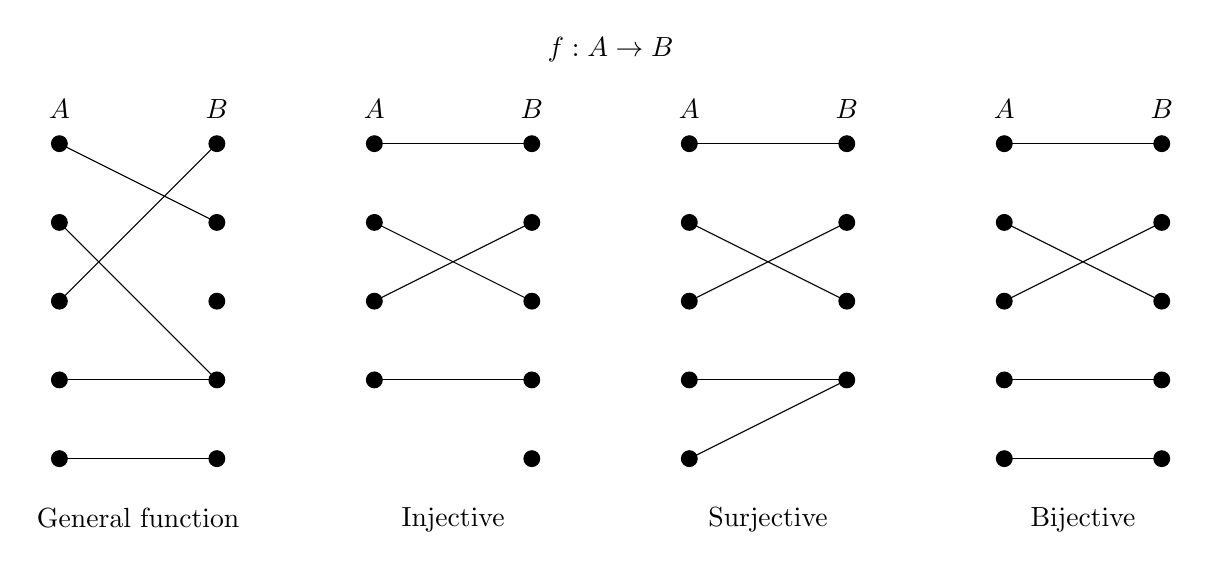
\begin{tikzpicture}
%\draw [lightgray, ultra thin] (0,0) grid (15,6);

\node at (7,6.2) {\(f:A\to B\)};

\draw [fill=black] (0,5) circle [radius=0.1];
\draw [fill=black] (0,4) circle [radius=0.1];
\draw [fill=black] (0,3) circle [radius=0.1];
\draw [fill=black] (0,2) circle [radius=0.1];
\draw [fill=black] (0,1) circle [radius=0.1];
\draw [fill=black] (2,5) circle [radius=0.1];
\draw [fill=black] (2,4) circle [radius=0.1];
\draw [fill=black] (2,3) circle [radius=0.1];
\draw [fill=black] (2,2) circle [radius=0.1];
\draw [fill=black] (2,1) circle [radius=0.1];
\node [above] at (0,5.2) {\(A\)};
\node [above] at (2,5.2) {\(B\)};
\node [below] at (1,0.5) {General function};

\draw [->] (0,5) -- (2,4);
\draw [->] (0,4) -- (2,2);
\draw [->] (0,3) -- (2,5);
\draw [->] (0,2) -- (2,2);
\draw [->] (0,1) -- (2,1);

\draw [fill=black] (4,5) circle [radius=0.1];
\draw [fill=black] (4,4) circle [radius=0.1];
\draw [fill=black] (4,3) circle [radius=0.1];
\draw [fill=black] (4,2) circle [radius=0.1];

\draw [fill=black] (6,5) circle [radius=0.1];
\draw [fill=black] (6,4) circle [radius=0.1];
\draw [fill=black] (6,3) circle [radius=0.1];
\draw [fill=black] (6,2) circle [radius=0.1];
\draw [fill=black] (6,1) circle [radius=0.1];
\node [above] at (4,5.2) {\(A\)};
\node [above] at (6,5.2) {\(B\)};
\node [below] at (5,0.5) {Injective};

\draw [->] (4,5) -- (6,5);
\draw [->] (4,4) -- (6,3);
\draw [->] (4,3) -- (6,4);
\draw [->] (4,2) -- (6,2);

\draw [fill=black] (8,5) circle [radius=0.1];
\draw [fill=black] (8,4) circle [radius=0.1];
\draw [fill=black] (8,3) circle [radius=0.1];
\draw [fill=black] (8,2) circle [radius=0.1];
\draw [fill=black] (8,1) circle [radius=0.1];
\draw [fill=black] (10,5) circle [radius=0.1];
\draw [fill=black] (10,4) circle [radius=0.1];
\draw [fill=black] (10,3) circle [radius=0.1];
\draw [fill=black] (10,2) circle [radius=0.1];

\node [above] at (8,5.2) {\(A\)};
\node [above] at (10,5.2) {\(B\)};
\node [below] at (9,0.5) {Surjective};

\draw [->] (8,5) -- (10,5);
\draw [->] (8,4) -- (10,3);
\draw [->] (8,3) -- (10,4);
\draw [->] (8,2) -- (10,2);
\draw [->] (8,1) -- (10,2);

\draw [fill=black] (12,5) circle [radius=0.1];
\draw [fill=black] (12,4) circle [radius=0.1];
\draw [fill=black] (12,3) circle [radius=0.1];
\draw [fill=black] (12,2) circle [radius=0.1];
\draw [fill=black] (12,1) circle [radius=0.1];
\draw [fill=black] (14,5) circle [radius=0.1];
\draw [fill=black] (14,4) circle [radius=0.1];
\draw [fill=black] (14,3) circle [radius=0.1];
\draw [fill=black] (14,2) circle [radius=0.1];
\draw [fill=black] (14,1) circle [radius=0.1];
\node [above] at (12,5.2) {\(A\)};
\node [above] at (14,5.2) {\(B\)};
\node [below] at (13,0.5) {Bijective};

\draw [->] (12,5) -- (14,5);
\draw [->] (12,4) -- (14,3);
\draw [->] (12,3) -- (14,4);
\draw [->] (12,2) -- (14,2);
\draw [->] (12,1) -- (14,1);
\end{tikzpicture}
\end{center}
\end{document}